\documentclass[10pt]{beamer}

\newtheorem{thm}{Theorem}
\usetheme[progressbar=frametitle]{metropolis}
\usepackage{appendixnumberbeamer}

\usepackage{booktabs}
\usepackage[scale=2]{ccicons}

\usepackage{pgfplots}
\usepgfplotslibrary{dateplot}

\usepackage{xspace}
\newcommand{\themename}{\textbf{\textsc{metropolis}}\xspace}

\title{CS1101S}
\subtitle{Programming Methodology I}
% \date{\today}
\date{}
\author{Theodore Leebrant}
\institute{Studio 2 - Tutorial Group 8D}
% \titlegraphic{\hfill\includegraphics[height=1.5cm]{logo.pdf}}

\begin{document}

\maketitle

% \begin{frame}{Workflow}
%   \setbeamertemplate{section in toc}[sections numbered]
%   \tableofcontents%[hideallsubsections]
% \end{frame}

\section[Admin Stuff]{Admin}


\begin{frame}{Safety Measures}
\begin{itemize}
  \item Masks on at all time
  \item Stay 1.5m apart
  \item Passing objects require disinfection (e.g. markers)
  \item Take attendance and picture of seating arrangement
\end{itemize}
\end{frame}

\begin{frame}[fragile]{Attendance Taking}
\begin{centering}
\href{https://inetapps.nus.edu.sg/ctr/Session/Details/158206}{\underline{Click here for photo submission}} \\

\includegraphics[width=0.5\textwidth]{qrattendancestudio2.png} \\
We will take photo when everyone is present. \\
\end{centering}
\end{frame}

\begin{frame}[fragile]{Telegram Group}
\begin{center}
  
\includegraphics[width=0.5\textwidth]{teleqr.png} \\
  alternatively \href{https://t.me/joinchat/DJDbrBmLMZciD4D4Z_Bodw}{\underline{click here}}
\end{center}
\end{frame}

\begin{frame}[fragile]{About Me}
  \begin{itemize}
    \item Theodore Leebrant
    \item Year 2 Computer Science \& Mathematics + USP
    \item Living in Cinnamon College
    \item Telegram: \href{https://t.me/kagamination}{@\underline{kagamination}}
    \item Email: \href{mailto:theodoreleebrant@u.nus.edu}{\underline{theodoreleebrant@u.nus.edu}}
  \end{itemize}
\end{frame}

\begin{frame}[fragile]{Introduce Yourself!}
  \begin{itemize}
    \item Preferred name
    \item Major (Probably CS)
    \item Academic and Programming Background
    \item Where do you stay?  \\ Halls, RCs, Woodlands, Johor, Japan, Yishun, or elsewhere
    \item Why CS (or your major)?
  \end{itemize}
\end{frame}

\begin{frame}[fragile]{About This Studio}
\begin{itemize}
  \item Safe space
  \begin{itemize}
    \item Questions, mistakes, comments are welcome.
  \end{itemize}
  \item Expectations
  \begin{itemize}
    \item \textbf{Come to studio prepared for discussion!}
    \item (Try to) finish the studio sheet.
    \item If still cannot, at least read the questions. 
  \end{itemize}
  \item Workflow
  \begin{itemize}
    \item We will start 5 minutes late or when 6/8 people comes, whichever earlier
    \item 5 minutes for admin (attendance taking, path/mission/quest review)
    \item 10 minutes for lecture and brief recap
    \item The rest for studio sheet
    \item I'll stay back for any questions if needed
  \end{itemize}
\end{itemize} 
\end{frame}


\begin{frame}[fragile]{Communication Channels}
  \begin{itemize}
    \item LumiNUS announcements
    \begin{itemize}
      \item Look out for this, profs will send general announcements
    \end{itemize}
    \item Piazza
    \begin{itemize}
      \item A forum for general questions. Use it to ask questions; if you have free time, you can go ahead and answer questions there.
    \end{itemize}
    \item Emails
    \begin{itemize}
      \item For more official stuff, e.g. submitting MCs if you are absent.
    \end{itemize}
    \item Telegram (group)
    \begin{itemize}
      \item For less official stuff, e.g. asking questions or sharing memes. You are welcome to PM me if you feel uncomfortable talking in the group.
    \end{itemize}
  \end{itemize}
\end{frame}

\begin{frame}[fragile]{Consultations}
  \begin{itemize}
    \item PM me on Telegram (preferred) or drop an email
    \item Either group or 1-to-1 consultations are fine, keep it below 5 people.
    \item F2F (preferred) or online (through zoom/discord)
    \item Check for timing, at least 1 day ahead. Most free on Mondays.
  \end{itemize}
\end{frame}

\begin{frame}[fragile]{Code of Honor}
  \begin{itemize}
    \item My answers to homework, quizzes, exams, and contests will be my own work (except for assignments that explicitly permit collaboration).
    \item My answers to paths, missions, and quests are \textbf{written by myself.} I am allowed to discuss ideas and algorithms with other students, but will work out the actual solution myself.
    \item I will not make solutions to homework, quizzes or exams available to anyone else. This includes both solutions written by me, as well as any official solutions provided by the course staff.
    \item I will not engage in any other activities that will dishonestly improve my results or dishonestly improve/hurt the results of others.
  \end{itemize}
\end{frame}

\begin{frame}[fragile]{How to do Missions and Quests}
  \textbf{Stuck?}
  \begin{itemize}
    \item Try to figure it out by yourself for another 30 minutes.
    \item Ask your fellow cadets
    \begin{enumerate}
      \item Studio telegram group
      \item Piazza
      \item etc.
    \end{enumerate}
    \item Let me know, maybe the question is wrong.
  \end{itemize}
\end{frame}

\begin{frame}[fragile]{Avenger Grading}
  \begin{itemize}
    \item Missions and Quests 
    \begin{itemize}
      \item Marked by me
      \item 18\% of your grades from the XPs
      \item Resubmissions allowed in the spirit of learning (ask me to unsubmit)
    \end{itemize}
    \item Studio grading (5\%)
    \begin{itemize}
      \item Show up for attendance marks
      \item Try to answer questions for particpation but no competition
      \item Participation is not about looking smart or getting problems right
      \item Make your mistakes here (instead of in the exams)
      \item Help your fellow studio cadets if they struggle
    \end{itemize}
    \item Mastery Checks ($3\% \times 2$)
    \begin{itemize}
      \item Two checks on your learning progress during the semester
      \item Form pairs and schedule appointment
      \item MC1: Weeks 4-13, MC2: Weeks 9-13
      \item 3 topics, 5 minutes per person per topic, Pass/Fail
      \item Re-testing allowed.
    \end{itemize}
  \end{itemize}
\end{frame}

\begin{frame}[fragile]{Studio Grading}
Out of 500XP per session:
  \begin{itemize}
    \item 200 for attendance (warm body)
    \item Reasonable contribution brings you up to 350
    \item Exceptional contribution brings you up to 400
    \item Replace me as TA to get 500
  \end{itemize}
Remember: XP comes from many sources.
\end{frame}

\section[Recap]{Recap}

{%
\setbeamertemplate{frame footer}{*This "something" is a valid combination of operands and operators.}
\begin{frame}[fragile]{Expressions vs. Statements}
  \begin{itemize}
    \item Expressions: \\
    \begin{itemize}
      \item Something* that can be \textbf{evaluated}.
      \item Examples: \verb|5| is an expression, \verb|3+4| is also an expression.
    \end{itemize}

    \item Statements: \\
    \begin{itemize}
      \item Programs that can be \textbf{executed}
      \item Will trigger a computational process.
      \item One statement is the expression statement, i.e. an expression followed by semicolon. For example: \verb|5;| is a statement.
    \end{itemize}

  \end{itemize}  
  Related piazza post: \href{https://piazza.com/class/kas136yscf8605?cid=79}{\underline{click here}}
\end{frame}
}

\begin{frame}[fragile]{Operators and Operands}
  Operators act on operands. \\
  Examples:
  \begin{itemize}
    \item \texttt{-5}
    \item \verb|!true|
    \item \verb|2 + 3|
    \item \verb|first >= second|
    \item \verb|a && b|
    \item \verb|x ? y : z| (conditional expression)
  \end{itemize}  
\end{frame}

\begin{frame}[fragile]{Constants and Functions}
  \begin{itemize}
    \item Constant declaration
    \item Function declaration and application
    \item Function parameters and arguments \\
  \end{itemize}  
    Example: \href{https://share.sourceacademy.nus.edu.sg/constfunc}{\underline{https://share.sourceacademy.nus.edu.sg/constfunc}} \\
\begin{verbatim}
const x = 5;
function cube(num) {
    return num * num * num;
}
cube(3);
cube(x);
\end{verbatim}
\end{frame}

\begin{frame}[fragile]{Environments and Conditional expressions}
Environment: a mechanism that allows naming.
Example: \href{https://share.sourceacademy.nus.edu.sg/conditionalexpressions}{\underline{https://share.sourceacademy.nus.edu.sg/conditionalexpressions}} \\
\begin{verbatim}
const age = 25;
age > 21 ? "can vote" : "cannot vote";
\end{verbatim}
General form: \verb|predicate ? consequent expression : alternate expression|
\end{frame}

\begin{frame}[fragile]{Abstraction}
Thinking at a higher level - you don't need to know how it works under the hood. \\

Classic example: car; has a lot of components, but you just use the car and drive. \\

CS1101S example: \texttt{mosaic} function re-used in mission 1 question 3 and 4. You don't need to care how it is implemented. \href{https://share.sourceacademy.nus.edu.sg/abstraction}{\underline{Example.}}
\end{frame}

\section[Studio Sheet (and Photo Taking)]{Studio Sheet}

\section[Additional Material]{Additional Material}
\begin{frame}[fragile]{Mission Feedback}
Most of you got the idea of what to do in missions, so keep up the good work. \\

In general, if I flag an issue, it's something that needs to be addressed. Try to follow the Source styling guide available \href{https://source-academy.github.io/source/source_styleguide.pdf}{\underline{here}} for reference on how to make your code readable in terms of indentation and spacing. For parameter naming, try to have concise but meaningful names - there is a tradeoff between verbosity and readability.
\end{frame}

\begin{frame}[fragile]{Mission Feedback - Commenting Style}
\begin{centering}
  \href{https://share.sourceacademy.nus.edu.sg/8h}{Example}
\end{centering}
\begin{itemize}
  \item Comments about the function goes above the function
  \begin{itemize}
    \item You may use \verb|/* ... */| or the single line comment \verb|//|.
  \end{itemize}
  \item Comments about single line goes either above the line or on the line.
\end{itemize}   
\end{frame}

\begin{frame}[fragile]{Nugget N1: Evaluation of Expressions}
\texttt{(2+(4*6))*(3+12)} \\
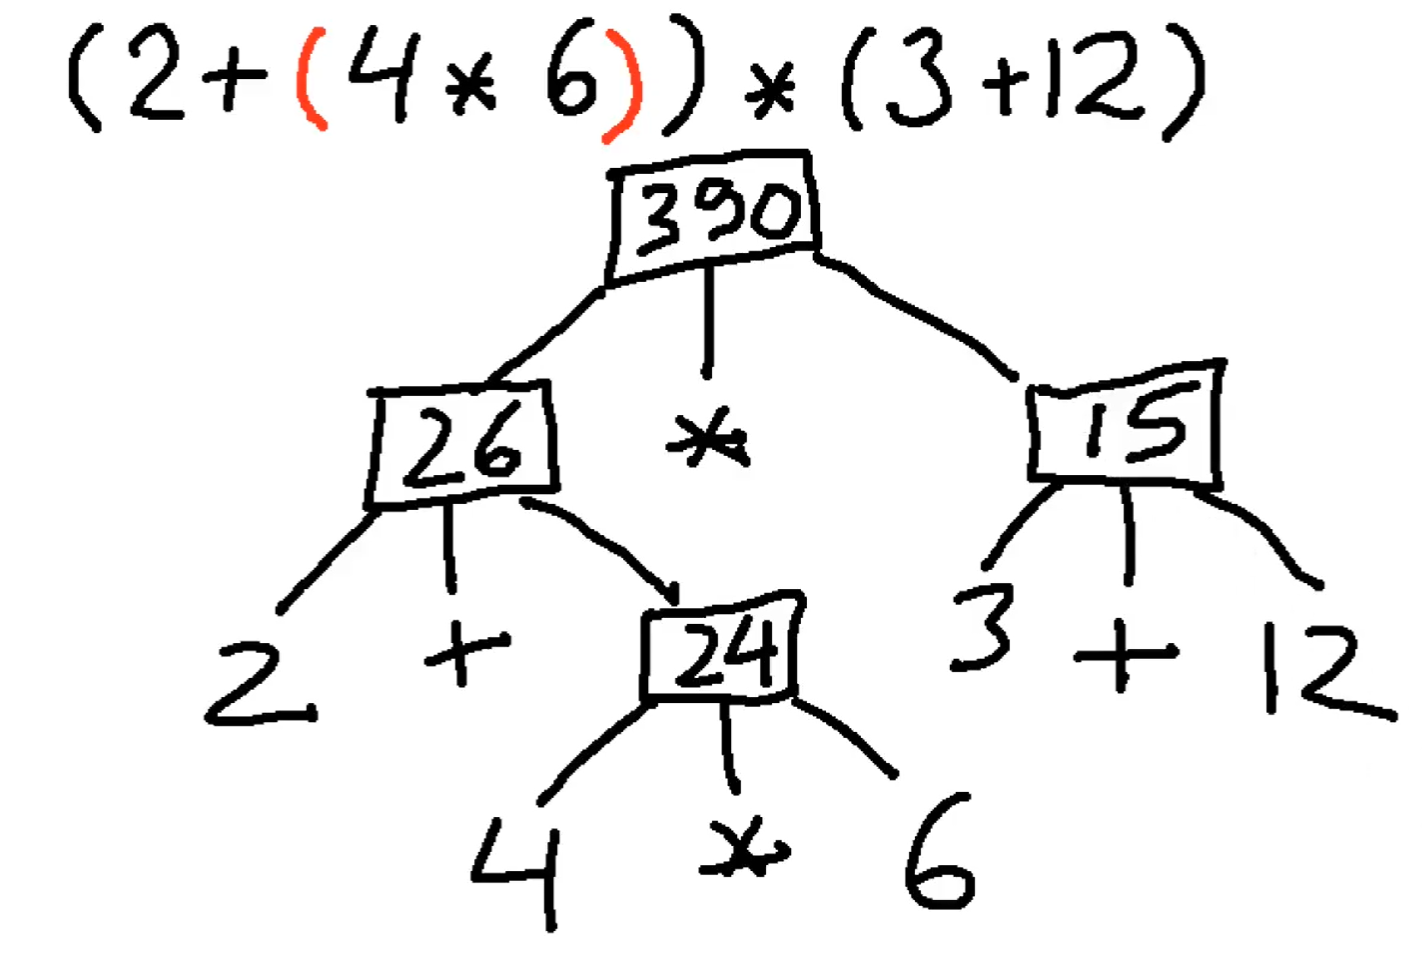
\includegraphics[width=0.7\textwidth]{tree.png}

Click \href{https://youtu.be/X7v8MGhn_cc}{\underline{here}} for visualisation.
\end{frame}
\end{document}
